% !TEX program = xelatex
% !TEX encoding = UTF-8  (utf8)

%\documentclass[glossy]{beamer}
\documentclass[glossy,handout]{beamer}

\mode<presentation>{
	\useoutertheme{wuerzburg}
	\useinnertheme[realshadow,corners=2pt,padding=2pt]{chamfered}
	\usecolortheme{shark}
	\usefonttheme{serif}
	\usefonttheme{professionalfonts}
	\usefonttheme{structurebold}
}

%%%%% fontspec
\usepackage{fontspec}
\setmainfont[BoldFont={Georgia Bold},
	ItalicFont={Georgia Italic},
	BoldItalicFont={Georgia Bold Italic}
	]{Georgia}

%%%%% XeCJK
\usepackage[AutoFallBack,AutoFakeBold,AutoFakeSlant,
	PunctStyle=CCT]{xeCJK}
\setCJKmainfont[%BoldFont={Adobe Heiti Std},
	ItalicFont={Adobe Kaiti Std},
%	SlantedFont={Adobe Song Std},
    BoldItalicFont={Weibei SC},
%    BoldSlantedFont={Adobe Fangsong Std}
	]{Adobe Heiti Std}
%\usepackage{xeCJKfntef}		%汉字加点和可断行的下划线
\setCJKmathfont{Cambria Math}

%%%%% math settings
\usepackage{amsmath}		%数学环境,align, align*
\usepackage{amsfonts}		%数学字体,mathbb
\usepackage{amssymb}		%数学公式
%\usepackage{amsthm}			%已包含在amsmath中
%\usepackage{mathrsfs}		%数学花体
\usepackage{extarrows}		%\xlongequal
\usepackage{bm}				%bm

\usepackage{xcolor}

\usepackage{graphics}
\usepackage{graphicx}		%definecolor, colorbox, fcolorbox

\usepackage{ulem}			%各种下划线:uline, uuline, uwave, sout, xout
%\usepackage{enumerate}
%\usepackage{esint}			%any type of integral symbol
% \usepackage{tabularx}
% \usepackage{multirow}
% \usepackage{verbatim}
% \usepackage{listings}
%\usepackage{polynom}		%多项式的竖式带余除法
%\usepackage{overpic}		%允许在图片上写文字
%\usepackage{wrapfig}		%支持插入文字环绕的图片
\usepackage{booktabs}		%粗的表格横线

\usepackage{tcolorbox} 		%各种自定义的盒子
\tcbuselibrary{skins, breakable, theorems}

\usepackage{tikz}
\usetikzlibrary{shapes,arrows,positioning,matrix,chains,backgrounds,fit}
\newcommand<>{\hover}[1]{
	\uncover#2{%
	\begin{tikzpicture}[remember picture,overlay]%
	\draw[fill,opacity=0.4] (current page.south west)
	rectangle (current page.north east);
	\node at (current page.center) {#1};
	\end{tikzpicture}}
}

\title{作业讲评}
\author{YB. Tang}
\institute{NUDT}
%\date{\today}
\date{2018-AU}

\begin{document}

%%%%% my macros
%===============macros====================
\def\ds{\displaystyle}
% \def\fin{\hfill$\Box$}
\def\fin{\hfill{\color{green!50!black}$\blacksquare$}}
\def\bs{\bigskip}
\def\b{\color{blue!80!yellow}}
\def\bb{\bf\color{blue}}
\def\e{\ensuremath{\varepsilon}}

\newcommand{\ba}[1]{\alert{\bf #1}}
\providecommand{\mbb}[1]{\ensuremath{\mathbb{{#1}}}}
\providecommand{\mr}[1]{\ensuremath{\mathrm{{#1}}}}


\newcommand{\limn}{\ensuremath{\lim\limits_{n\to\infty}}}
\newcommand*{\limx}[1]{\ensuremath{\lim\limits_{x\to{#1}}}}
\newcommand*{\limdx}{\ensuremath{\lim\limits_{\Delta x\to 0}}}
\providecommand{\llim}[1]{\ensuremath{\lim\limits_{#1}}}

\newcommand{\sumn}[1][1]{\ensuremath{\sum\limits_{n=#1}^{\infty}}}
\providecommand{\sumk}[1]{\ensuremath{\sum\limits_{k={#1}}^n}}
\providecommand{\suml}{\ensuremath{\sum\limits}}

\newcommand*{\df}[2]{\displaystyle\frac{\,{#1}\,}{\,{#2}\,}}
\newcommand*{\dx}{\Delta x}
\renewcommand{\d}{\mathrm{d}}
\newcommand*{\p}{\ensuremath{\partial}}

\newcommand{\dint}{\ensuremath{\displaystyle\int}}

\newcommand{\ps}[1]{$^{[\mbox{\kaiti\footnotesize 注}]}$
\marginpar{\kaiti\small\color{blue} {注:}#1}}

%define tab of .25 textwidth and can auto strech
%\tab{the word}\tab{another word}\tab{3rd one}
\newlength{\tabcont}
\newcommand{\tab}[1]{%
	\settowidth{\tabcont}{#1}%
	\ifthenelse{\lengthtest{\tabcont < .25\linewidth}}%
	{\makebox[.25\linewidth][l]{#1}\ignorespaces}%
	%{\makebox[.5\linewidth][l]{\color{red} #1}\ignorespaces}%
	{\makebox[.5\linewidth][l]{#1}\ignorespaces}%
}%

%set fontsize with number of points
% \newcommand{\fs}[1]{\fontsize{#1 pt}{5pt}\selectfont}

\newtcolorbox{thx}{colframe=blue!40!black,colback=white,breakable}

\newtcolorbox{ext}{colframe=green!60!black,colback=green!20!white,breakable}

\definecolor{shadecolor}{rgb}{0.9,0.9,0.9}

\renewcommand{\thefigure}{\thechapter.\arabic{figure}}

%% !TEX root = ../1-main-SL.tex
% !TEX encoding = UTF-8  (utf8)

\begin{frame}
	\centering
	\bf\Huge\color{purple} 习题1-2讲评\\[1cm]
	\small\color{gray}2018-10-24
\end{frame}

\section{说在前面}

\begin{frame}[t]\frametitle{说在前面}
	\linespread{1.8}
	\Large
    \begin{itemize}
    	\item 如何改错?
    	\begin{enumerate}
    		\item {\it\Large 多留空白...}
    		\item {\it\Large 要还是不要,划清界限...}
    	\end{enumerate}
    	\item 对还是错?
    	\begin{enumerate}
    		\item {\it\Large $\sqrt[3]{n+1}-\sqrt[3]{n}<\sqrt{n+1}-\sqrt{n}$.}
    		\item {\it\Large 要证$\limn(a_{n+1}-a_n)=0$,只需证明}
    		$$\limn\df{a_{n+1}}{a_n}=1.$$
    		\item {\it\Large $\{a_n\}$有界,故可设$\limn a_n=A$.}
    	\end{enumerate}
    \end{itemize}
\end{frame}

\section{参考解答}

\begin{frame}[t]\frametitle{1.用极限的定义证明}
\large
(1)$\limn\df{\sqrt{n^2+a^2}}n=1$;

证:\it 对任意$\e>0$,令$N=\left[\df{a^2}{\e}\right]+1>\df{a^2}{\e}$,
则对任意$n>N$,均有
$$\left|\df{\sqrt{n^2+a^2}}n-1\right|
=\df{a^2}{n(\sqrt{n^2+a^2}+n)}<\df{a^2}n<\df{a^2}N<\e,
$$
由数列极限的定义,即证。\fin
\end{frame}

\begin{frame}[t]\frametitle{1.用极限的定义证明}
\large

(2)$\limn0.\underbrace{99\ldots9}_{n\mbox{\footnotesize 个}}=1.$

证:\it 对任意$\e>0$,令$N=[-\lg\e]+1$,则对任意$n>N$,均有
$$|0.\underbrace{99\ldots9}_{n\mbox{\footnotesize 个}}-1|
=\df1{10^n}<\df1{10^N}
<\df1{10^{-\lg\e}}=\e,$$
由数列极限的定义,即证。\fin
\end{frame}

\begin{frame}[t]\frametitle{1.用极限的定义证明}
\large

(3)$\limn\left(\sqrt[3]{n+1}-\sqrt[3]{n}\right)=0$.
\bs

证:\it 对任意$\e>0$,令$N=\left[1/\e\right]+1$,则对任意$n>N$,有
$$|\sqrt[3]{n+1}-\sqrt[3]{n}|
=\df1{(n+1)^{\frac{2}{3}}+(n+1)^{\frac13}n^{\frac13}+n^{\frac23}}
<\df1n<\df1N<\e.$$
由数列极限的定义,即证。\fin
\end{frame}

\begin{frame}[t]\frametitle{1.用极限的定义证明}
\large

(4)$\limn\df{n^2-n-1}{2n^2+2n-4}=\df12$.
\bs

证:\it 对任意$\e>0$,令$N=$,则对任意$n>N$有
$$\left|\df{n^2-n-1}{2n^2+2n-4}-\df12\right|
=\left|\df{-2n-3}{2n^2+2n-4}\right|<\df1n<\df1N<\df1{\e}.$$
由数列极限的定义,即证。\fin
\end{frame}

\begin{frame}[t]\frametitle{证明极限的性质}
\large
2.数列$\{a_n\}$有界,$\limn b_n=0$,证明:$\limn a_nb_n=0$。
\end{frame}

\begin{frame}{哪里不太对?}
	\centering
	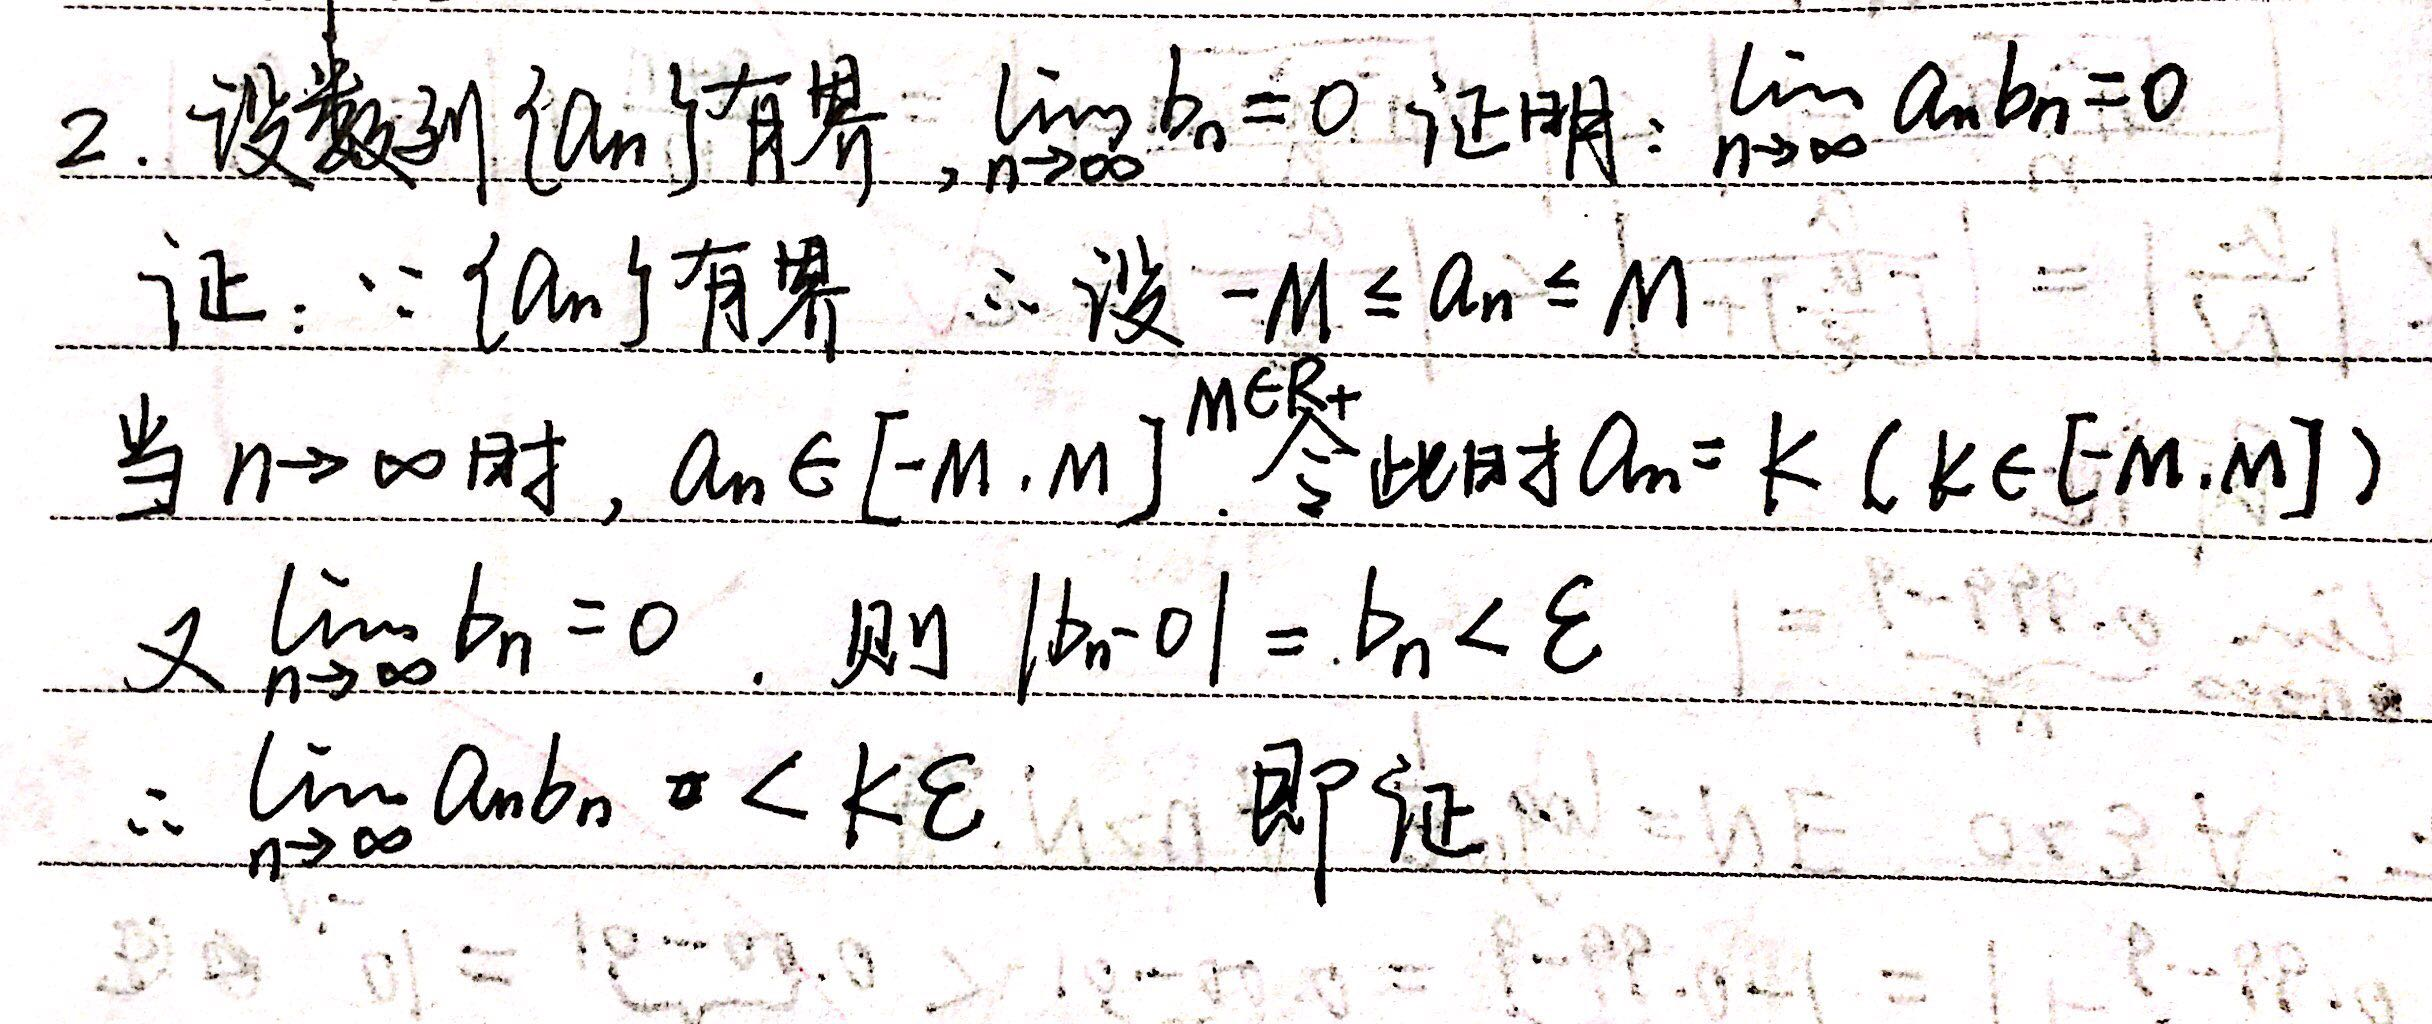
\includegraphics[width=0.9\textwidth]{./images/ch01/HWR/anbn0-1.jpeg}
\end{frame}

\begin{frame}{哪里不太对?}
	\centering
	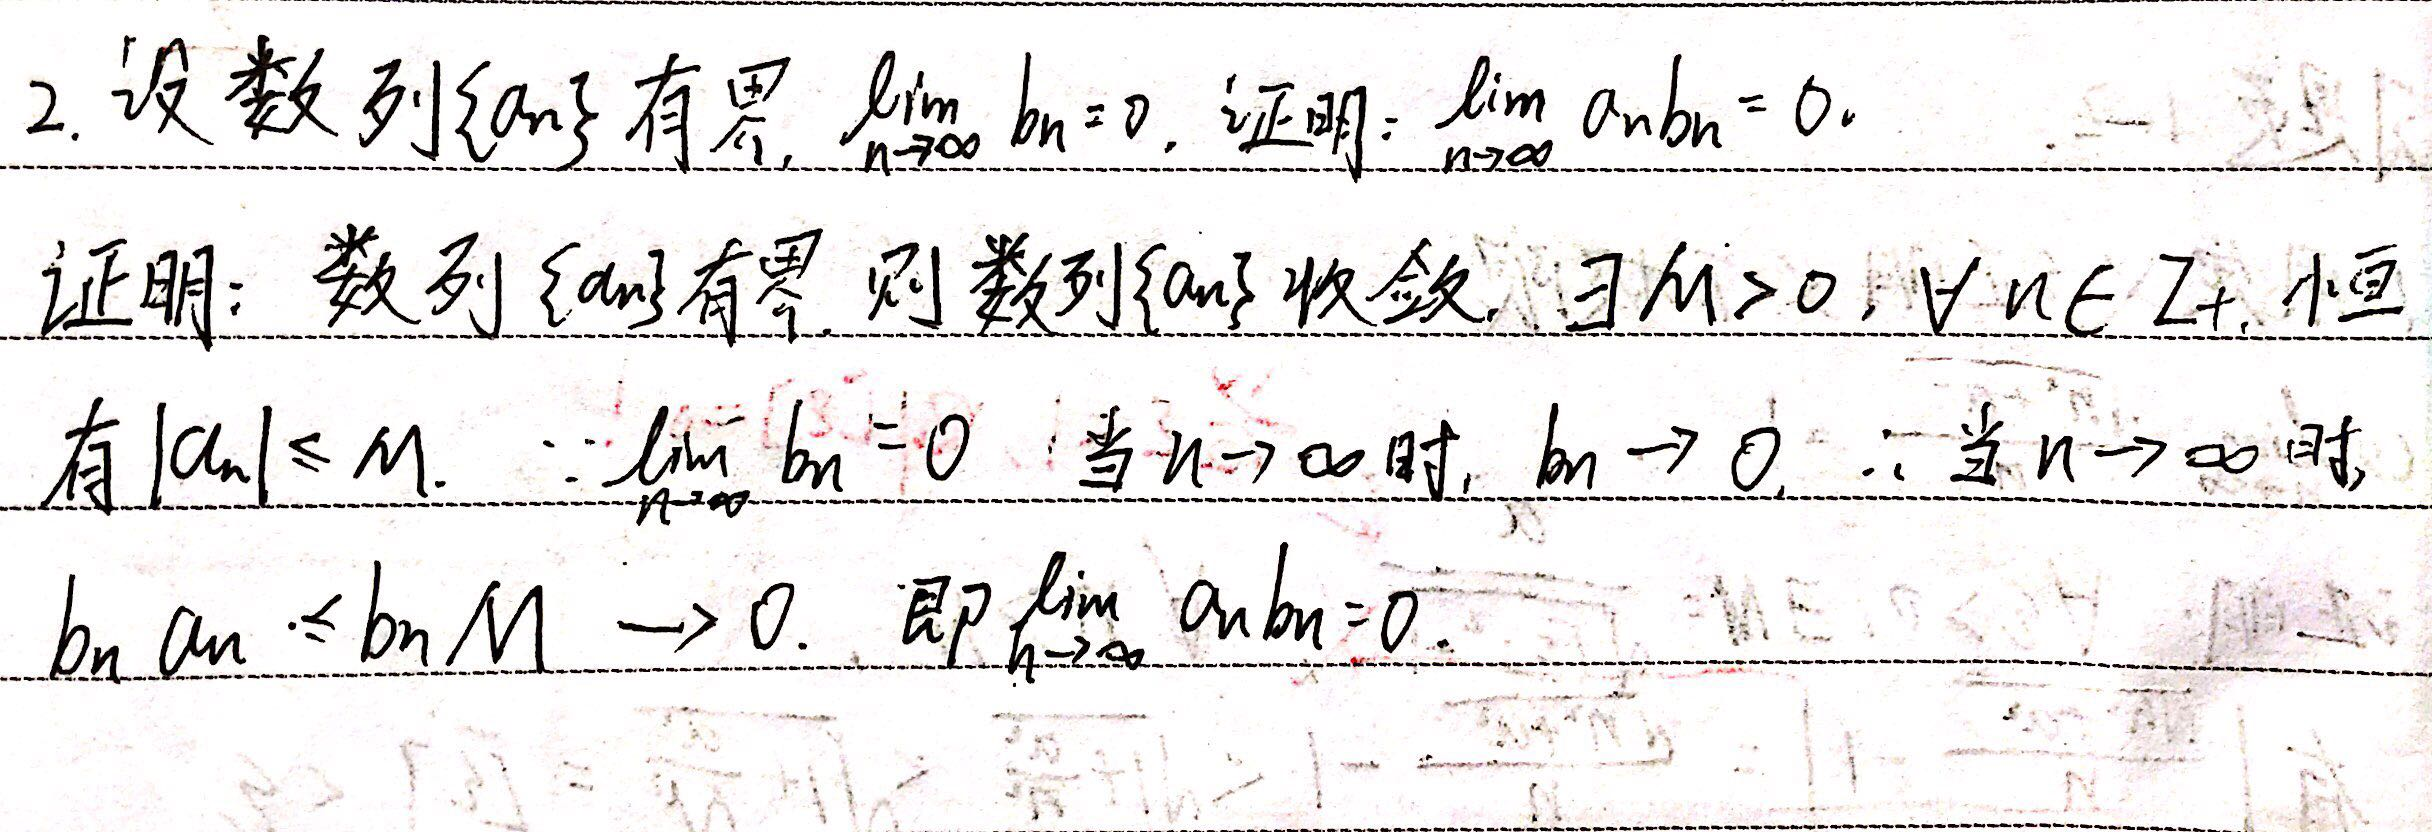
\includegraphics[width=0.9\textwidth]{./images/ch01/HWR/anbn0-2.jpeg}
\end{frame}

\begin{frame}{哪里不太对?}
	\centering
	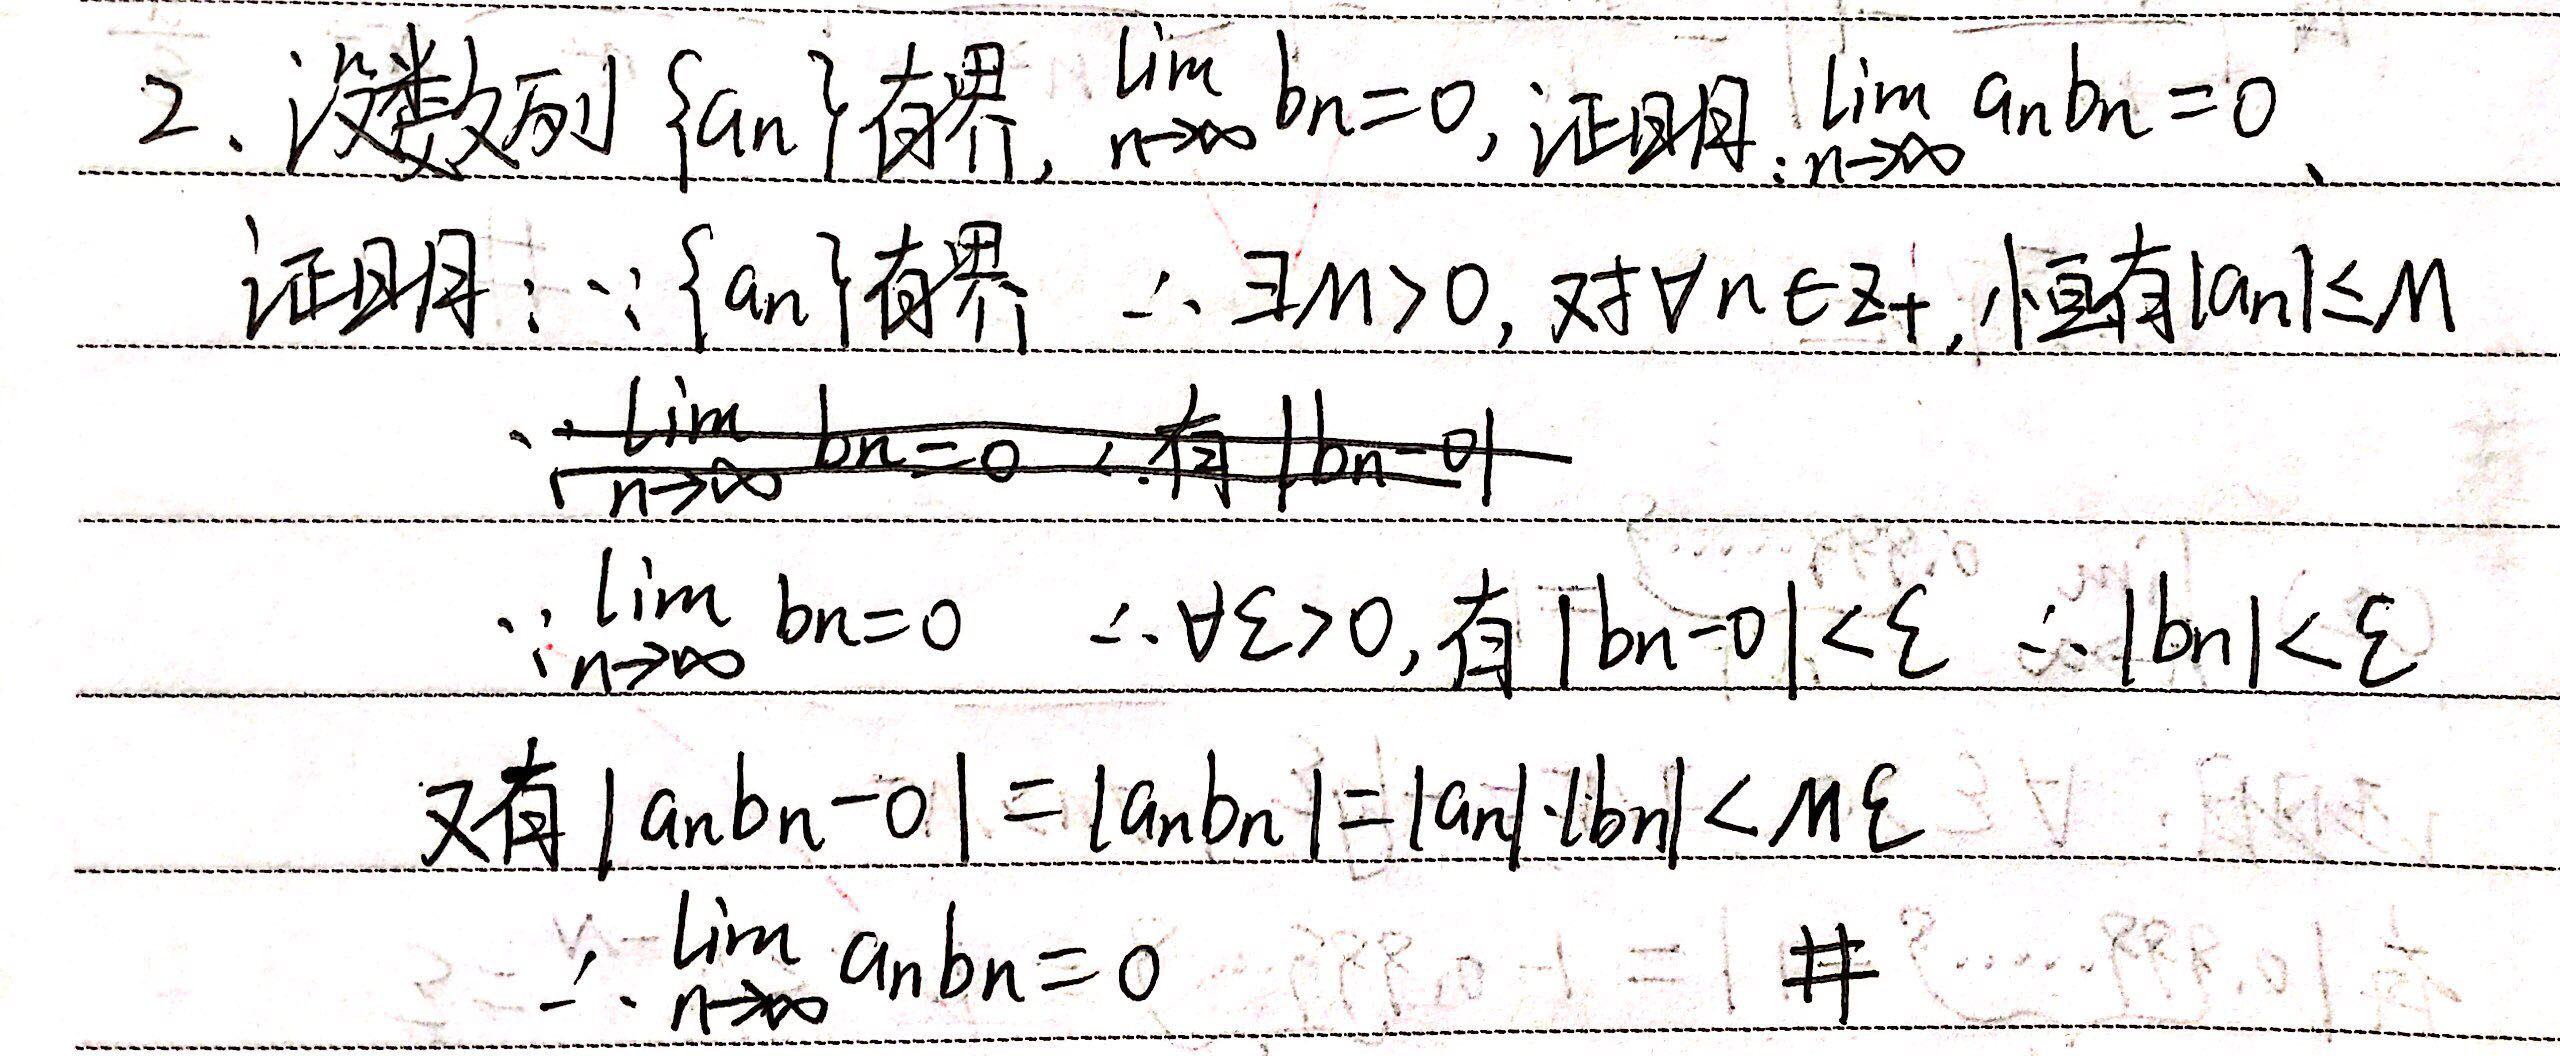
\includegraphics[width=0.9\textwidth]{./images/ch01/HWR/anbn0-3.jpeg}
\end{frame}

\begin{frame}{哪里不太对?}
	\centering
	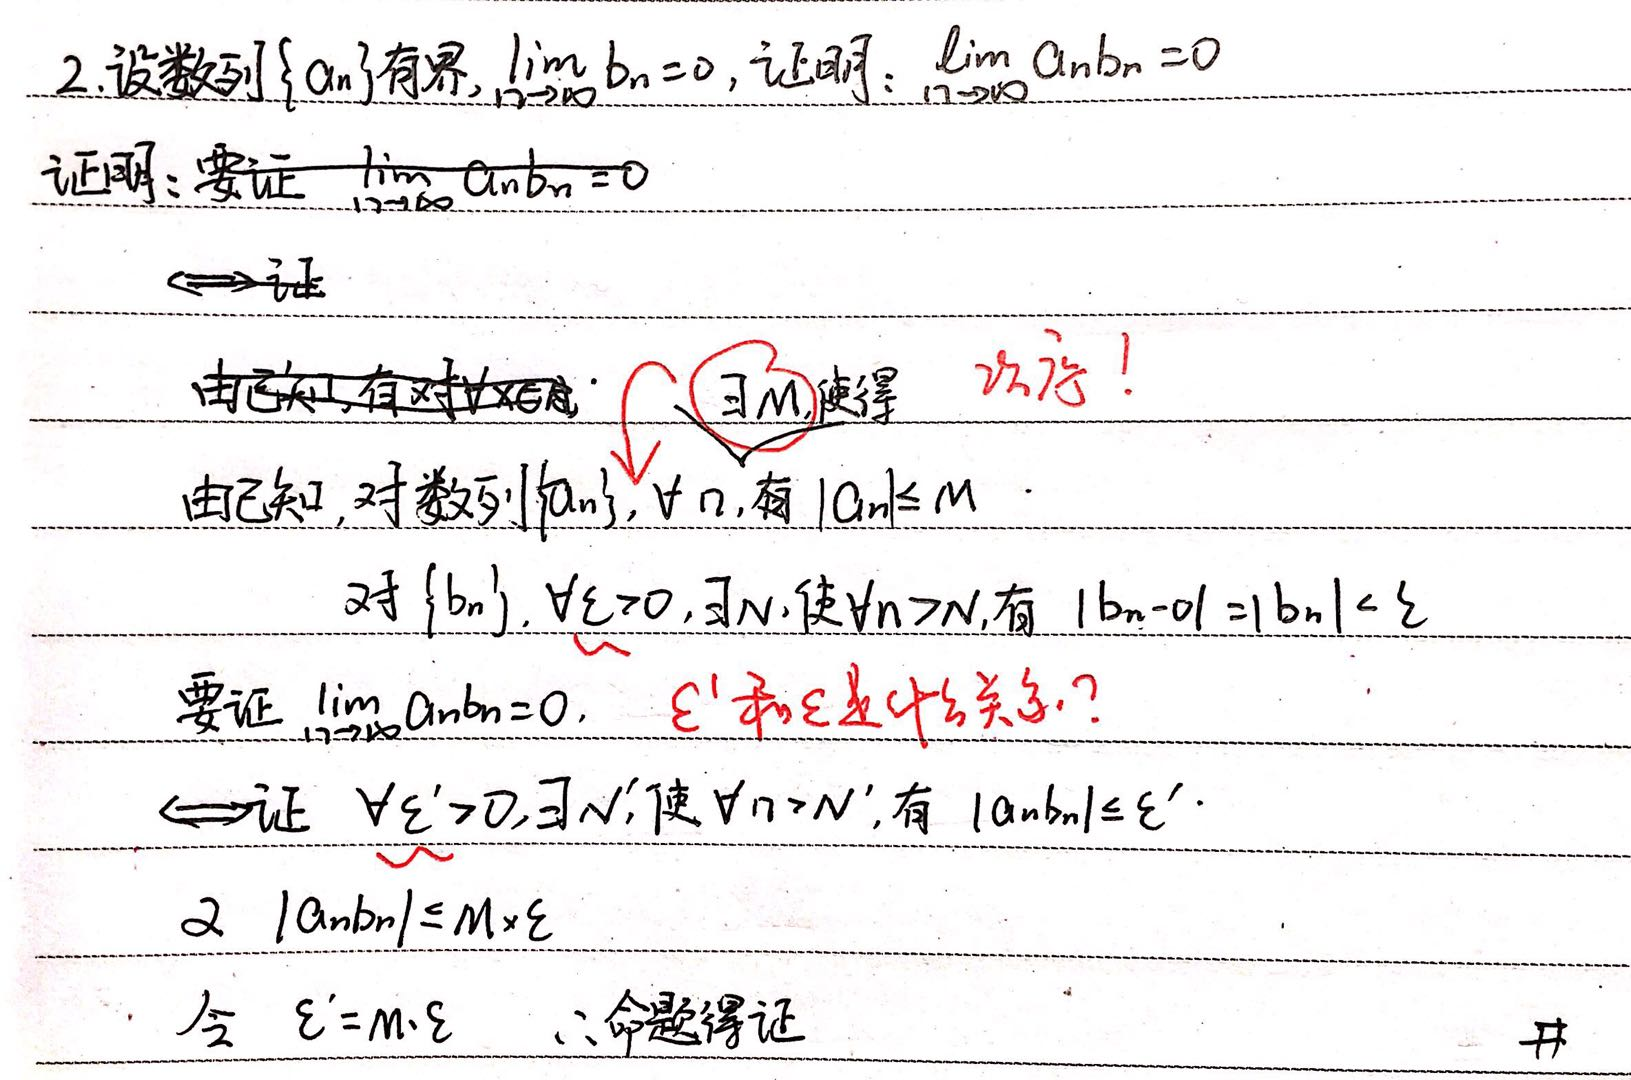
\includegraphics[width=0.9\textwidth]{./images/ch01/HWR/anbn0-4.jpeg}
\end{frame}

\begin{frame}[t]\frametitle{证明极限的性质}
\large
2.数列$\{a_n\}$有界,$\limn b_n=0$,证明:$\limn a_nb_n=0$。

证:\it 数列$\{a_n\}$有界,故存在$M>0$,对任意$n\in\mathbb{Z}_+$,均有
$$|a_n|\leq M.$$
对任意$\e>0$,令$\e_1=\df{\e}M$,由$\limn b_n=0$,存在$N$,对任意$n>N$有
$$|b_n-0|<\e_1.$$
综上,当$n>N$时,总有
$$|a_nb_n-0|\leq M\e_1=\e,$$
由数列极限的定义,即证。\fin
\end{frame}

\begin{frame}[t]\frametitle{证明极限的保号性}
\large
3.设$\limn a_n=a\ne 0$,证明:存在$N\in\mathbb{Z}^+$,对任意
$n>N$,有$|a_n|>|a|/2$。

证:\it 对$\e=\df{|a|}2$,由$\limn a_n=a$,存在$N\in\mathbb{Z}^+$,
对任意$n>N$,有
$$|a_n-a|<\e=\df{|a|}2.$$
由绝对值不等式$|a_n-a|>||a_n|-|a||$,故
$$||a_n|-|a||<\df{|a|}2.$$
也即
$$-\df{|a|}2<|a_n|-|a|<\df{|a|}2,$$
由其中的右侧不等式可知$|a_n|>\df{|a|}2$,即证。\fin
\end{frame}

\begin{frame}
	\centering
	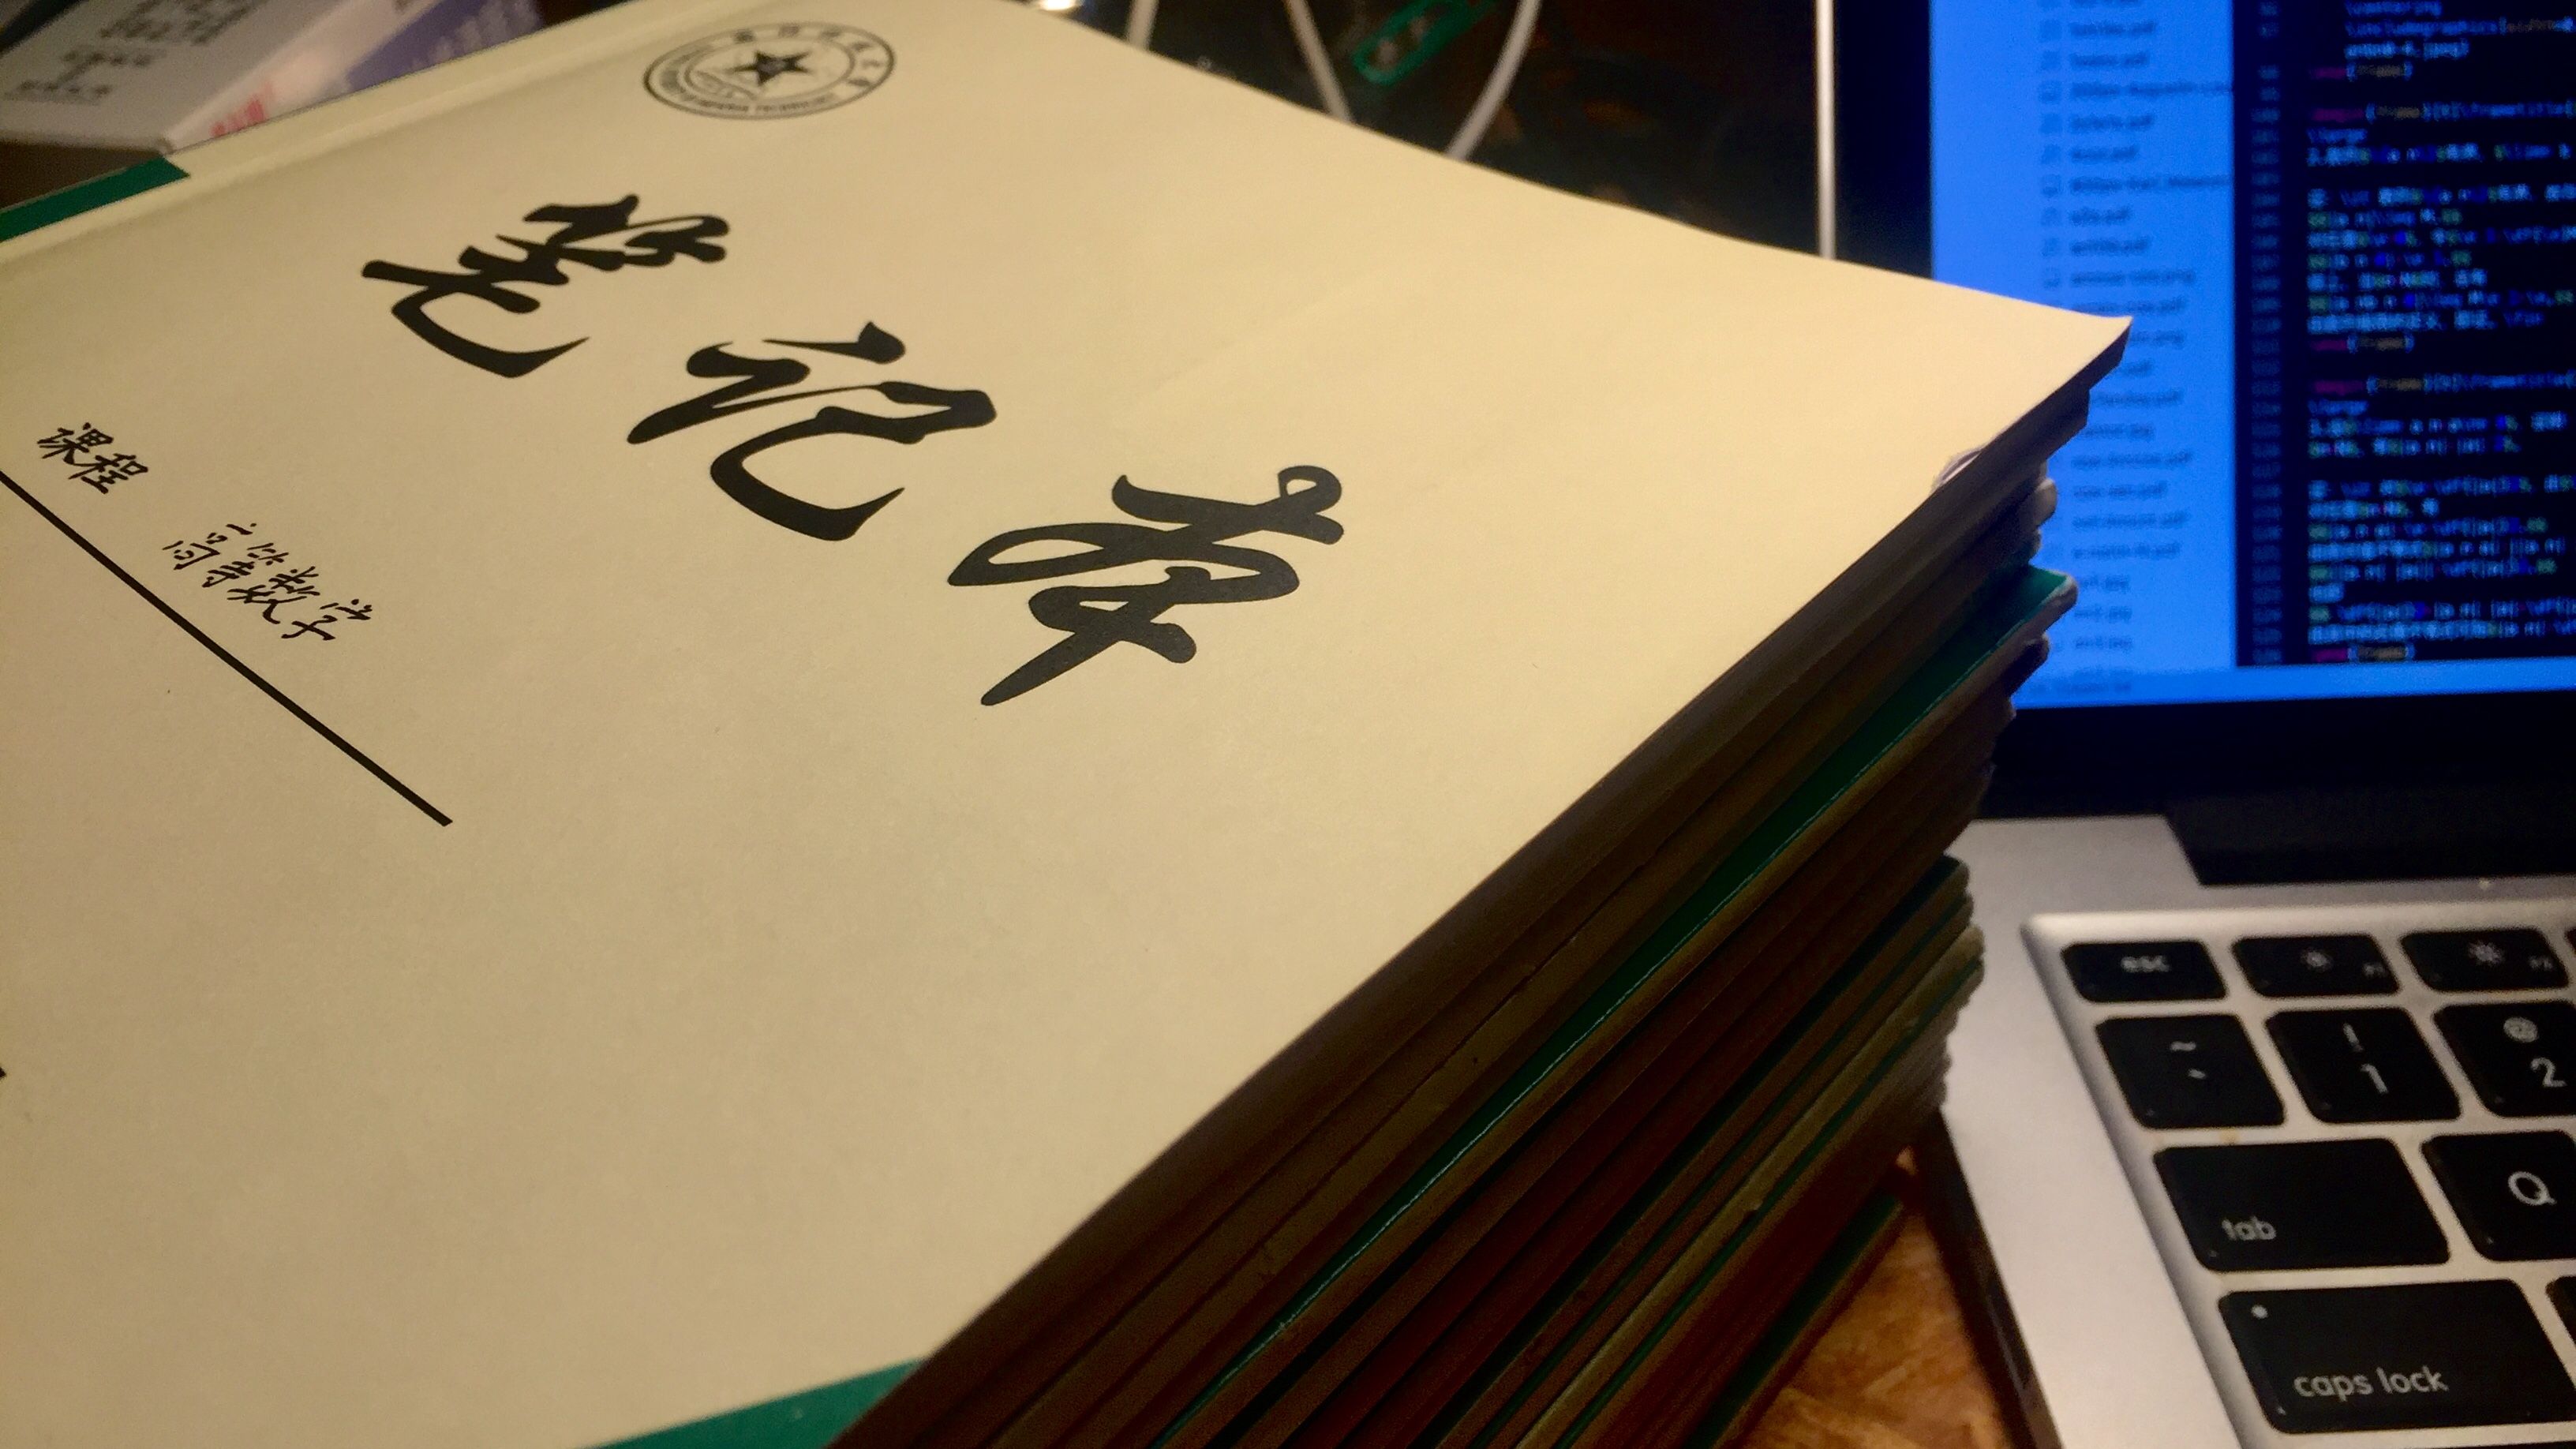
\includegraphics[width=0.9\textwidth]{./images/ch01/HWR/notebook.jpg}
\end{frame}

% !TEX root = ../1-main-SL.tex
% !TEX encoding = UTF-8  (utf8)

\begin{frame}
	\centering
	\bf\Huge\color{purple} 习题讲评\\[1em]
	\small 习题1-3 -- 习题1-5\\[1cm]
	\small\color{gray}2018-10-31
\end{frame}

\section{说在前面}

\begin{frame}[t]\frametitle{说在前面}
	\linespread{1.8}
	\Large
	\vspace*{-1em}
    \begin{itemize}
    	\item 作业订正
    	\begin{enumerate}
    		\item {\it\Large\baa 不订正一律C,新作业不予批改}
    		\item {\it\Large 尽量就近订正}
    	\end{enumerate}
    	\item 关于雷同
    	\begin{enumerate}
    		\item {\it\Large 不要太明显,抄也要动脑子!}
    		\item {\it\Large\baa 发现明显的抄袭,相关人一律C}
    	\end{enumerate}
    	\item 几个小问题
    	\begin{enumerate}
    		\item {\it\Large 无意义的极限,如:
    		$\limx0\df1x$,$\limx{\infty}\arctan x$}
    		\item {\it\Large 求渐近线一定要仔细,避免遗漏}
    		\item {\it\Large 作业和笔记不要写在同一个本子上!}
    	\end{enumerate}
    \end{itemize}
\end{frame}

\section{参考解答}

\subsection{习题1-3}

\begin{frame}[t]\frametitle{1.用极限的定义证明}
\large
(1)$\limx{-2}{x^2}=4$

证:\it 对任意$\e>0$,令$\delta=\min\left\{1,\frac{\e}5\right\}$,
则对任意$x\in U_0(2,\delta)$,总有$|x+2|<5$,进而
$$|x^2-4|=|x-2||x+2|<5|x-2|<5\cdot\df{\e}5<\e,$$
由极限的定义,即证。\fin
\end{frame}

\begin{frame}[t]\frametitle{1.用极限的定义证明}
\large

(2)$\limx{+\infty}\df{\sin x}{\sqrt x}=0$.

证:\it 对任意$\e>0$,令$X=\df1{\e^2}$,则对任意$x>X$,总有
$$\left|\df{\sin x}{\sqrt x}-0\right|\leq\df1{\sqrt x}
<\df1{\sqrt X}=\e.$$
由函数极限的定义,即证。\fin
\end{frame}

\begin{frame}[t]\frametitle{1.用极限的定义证明}
\large

(3)$\limx{\infty}\df{x+\sin x}{x+\cos x}=1$.
\bs

证:\it 对任意$\e>0$,令$X=\sqrt2/\e-1$,则对任意$|x|>X$,总有
$$\left|\df{x+\sin x}{x+\cos x}-1\right|
=\df{|\sin x-\cos x|}{|x+\cos x|}
<\df{\sqrt2}{|x|-1}<\df{\sqrt2}{X-1}=\e,$$
由函数极限的定义,即证。\fin
\end{frame}

\begin{frame}[t]\frametitle{Dirichlet函数的极限}
\large

2.证明:$f(x)=xD(x)$仅当$x=0$时极限存在。($D(x)$表示Dirichlet函数)
\bs

证:\it 对任意$\e>0$,令$\delta=\e$,对任意$x\in U_0(0,\delta)$,
注意到$|D(x)|\leq 1$,故总有
$$|xD(x)-0|\leq |x|<\delta=\e,$$
由函数极限的定义,$\limx0f(x)=0$。
\end{frame}

\begin{frame}[t]\frametitle{Dirichlet函数的极限(续)}
\large
\it
以下证明对任意$x_0\ne 0$,$\limx{x_0}f(x)$不存在。

对任意$x_0\ne0$,总可以取一个有理数列$\{x_n^{(1)}\}$
和一个无理数列$\{x_n^{(2)}\}$,使得
$$\limn x_n^{(1)}=\limn x_n^{(2)}=x_0.$$
注意到
$$\limn f(x_n^{(1)})=\limn x_n^{(1)}=x_0
\ne 0=\limn f(x_n^{(2)}),$$
故由Henie定理可知,当$x\to x_0$时$f(x)=xD(x)$不收敛。\fin
\end{frame}

\subsection{习题1-4}

\begin{frame}[t]\frametitle{无界与无穷大}
\large
1.证明:函数$y=\df1x\sin\df1x$在区间$(0,1]$内无界,但不是$x\to0^+$
时的无穷大。

\bs
证:\it 先证该函数无界。对任意$M>0$,总可令$x_M=\df1{2([M]+1)\pi+\frac{\pi}2}$,
则
\begin{align*}
	y(x_M)&=\left(2([M]+1)\pi+\frac{\pi}2\right)
	\sin\left[2([M]+1)\pi+\frac{\pi}2\right]\\
	&=2([M]+1)\pi+\frac{\pi}2>M.
\end{align*}
由函数无界的定义,即证。
\end{frame}

\begin{frame}[t]\frametitle{无界与无穷大(续)}
\large
\it 下证该函数不是$x\to0^+$时的无穷大。用反证法,若该函数是$x\to0^+$时的
无穷大,则$\limx{0^+}\df1y=0$。
考虑数列$x_n=\frac1{n\pi}$,显然$\limn x_n=0$,且$\sin\df1{x_n}=0$,
进而可知$\limn y(x_n)=0$。于是由Henie定理:
\begin{align*}
	1&=\limn y(x_n)\df1{y(x_n)}
	=\limn y(x_n)\limn\df1{y(x_n)}\\
	&=\limn y(x_n)\limx{0^+}\df1{y(x)}=0,
\end{align*}
显然不成立,由此即知假设错误,即证。\fin
\end{frame}

\begin{frame}[t]\frametitle{渐近线}
\large
2.求函数$y=\df1{1-x^2}$的水平渐近线和铅直渐进线。

解:\it 因为$\limx{\infty}y(x)=0$,故$x=0$是$y=\df1{1-x^2}$的水平渐近线;

又因为$\limx{\pm1}\df1{y(x)}=\limx{\pm1}(1-x^2)=0$,
故$y=\pm1$是$y=\df1{1-x^2}$的铅直渐近线。\fin

\centering
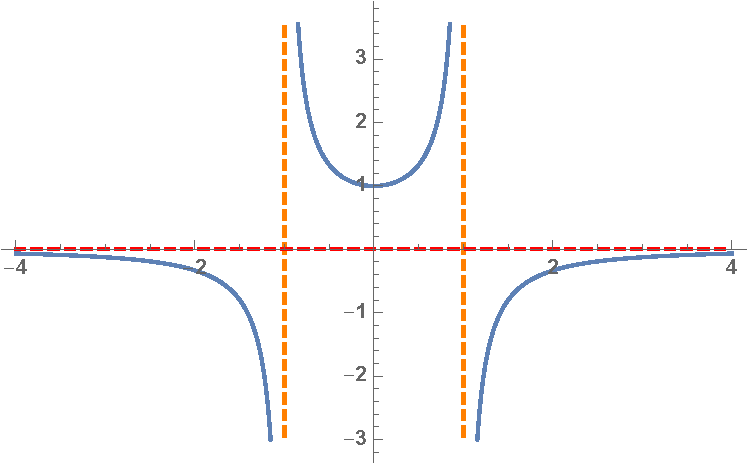
\includegraphics[width=0.6\textwidth]
{./images/ch01/11-x2.pdf}
\end{frame}

\subsection{习题1-5}

\begin{frame}[t]\frametitle{1. 计算如下极限}
\large
(1)
\begin{align*}
	\limx{1}&\left(\df1{1-x}-\df3{1-x^3}\right)
	=\limx1\df{(x-1)(x+2)}{(1-x)(1+x+x^2)}\\
	&=-\limx1\df{x+2}{1+x+x^2}=-1
\end{align*}

(2)
\begin{align*}
	\limx0&\df{(h+x)^3-h^3}x
	=\limx0\df{3h^2x+3hx^2+x^3}{x}\\
	&=\limx0(3h^2+3hx+x^2)=3h^2
\end{align*}
\end{frame}

\begin{frame}[t]\frametitle{1. 计算如下极限}
\large
(3)$\limx{\infty}\df{\arctan x}{x^2}$

解:{\it 因为$\limx{\infty}\df1{x^2}=0$,$|\arctan x|\leq\df{\pi}2$,
故由无穷小的性质可知:$\mbox{原式}=0.$}

\bs
(4)
\begin{align*}
	\limx{+\infty}&\df{\sqrt[3]{x+\sqrt{x+x^3}}}{\sqrt{x+1}}
	=\limx{+\infty}\df{\sqrt[3]{x^{-\frac16}
	+\sqrt{x^{-\frac13}+1}}}{\sqrt{1+x^{-1}}}\\
	&=\df{\sqrt[3]{\limx{+\infty}x^{-\frac16}
	+\sqrt{\limx{+\infty}x^{-\frac13}+1}}}{\sqrt{1+\limx{+\infty}x^{-1}}}=1.
\end{align*}
\end{frame}

\begin{frame}[t]\frametitle{1. 计算如下极限}
\large
(5)
\begin{align*}
	\limx4&\df{\sqrt{2x+1}-3}{\sqrt{x-2}-\sqrt2}
	=\limx4\df{(2x-8)(\sqrt{x-2}+\sqrt2)}{(x-4)(\sqrt{2x+1}+3)}
	=\df{2\sqrt2}3
\end{align*}

(6)
\begin{align*}
	\limx0&\df{\sqrt[3]{x+1}-1}x
	=\limx0\df{x}{x[(x+1)^{\frac{2}{3}}
	+3(x+1)^{\frac{1}{3}}+1]}
	=\df13
\end{align*}
\end{frame}

\begin{frame}[t]\frametitle{1. 计算如下极限}
\large
(7)
\begin{align*}
	\limx0&\df{\sqrt{1+x}+\sqrt{1-x}-2}{x^2}
	=\limx0\df{2(\sqrt{1-x^2}-1)}
	{x^2(\sqrt{1+x}+\sqrt{1-x}+2)}\\
	&=\limx0\df{-2x^2}{x^2(\sqrt{1+x}+\sqrt{1-x}+2)
	(\sqrt{1-x^2}+1)}=-\df14.
\end{align*}

(8)
\begin{align*}
	\limx{+\infty}&\df{\ln(2+e^{3x})}{\ln(3+e^{2x})}
	=\limx{+\infty}
	\df{3x+\ln(2e^{-3x}+1)}{2x+\ln(3e^{-2x}+1)}\\
	&=\limx{+\infty}
	\df{3+\df1x\ln(2e^{-3x}+1)}{2+\df1x\ln(3e^{-2x}+1)}
	=\df32
\end{align*}
\end{frame}

\begin{frame}[t]\frametitle{1. 计算如下极限}
\large
(9)
\begin{align*}
	\limx{+\infty}&x(\sqrt{x^2+1}-x)
	=\limx{+\infty}\df{x(\sqrt{x^2+1}+x)}{x^2}=\df12
\end{align*}

\bs
(10)$\limx{-\infty}x(\sqrt{x^2+1}-x)$

解:{\it 因为
$$\limx{-\infty}\df1{\sqrt{x^2+1}-x}
=\limx{-\infty}\df{1/x}{-\sqrt{1+x^{-2}}-1}=0,$$
故$x$和$\sqrt{x^2+1}-x$均为$x\to-\infty$时的
无穷大,从而可知该极限不存在。}
\end{frame}

\begin{frame}[t]\frametitle{1. 计算如下极限}
\large
(11)$\limx0x^2\sin\df1x$

解:{\it 因为$\limx0x^2=0$,$\left|\sin\df1x\right|\leq1$,由无穷小的性质,可知
$\mbox{原式}=0.$}
\end{frame}

\begin{frame}[t]\frametitle{利用极限的性质进行推导}
\large
2.确定常数$a,b$的值,使得
$\limx{\infty}\left(\df{x^2}{x+1}-ax-b\right)=0$。

解:\it
\begin{align*}
	0&=\limx{\infty}\left(\df{x^2}{x+1}-ax-b\right)\limx{\infty}\df1x
	=\limx{\infty}\df{\frac{x^2}{x+1}-ax-b}{x}\\
	&=\limx{\infty}\left(\df{x}{x+1}-a-\df bx\right)
	=1-a,
\end{align*}
故$a=1$,进而
\begin{align*}
	b&=\limx{\infty}\left(\df{x^2}{x+1}-x\right)
	=\limx{\infty}\df{-x}{x+1}=-1.
\end{align*}
\fin
\end{frame}

\begin{frame}
	\centering
	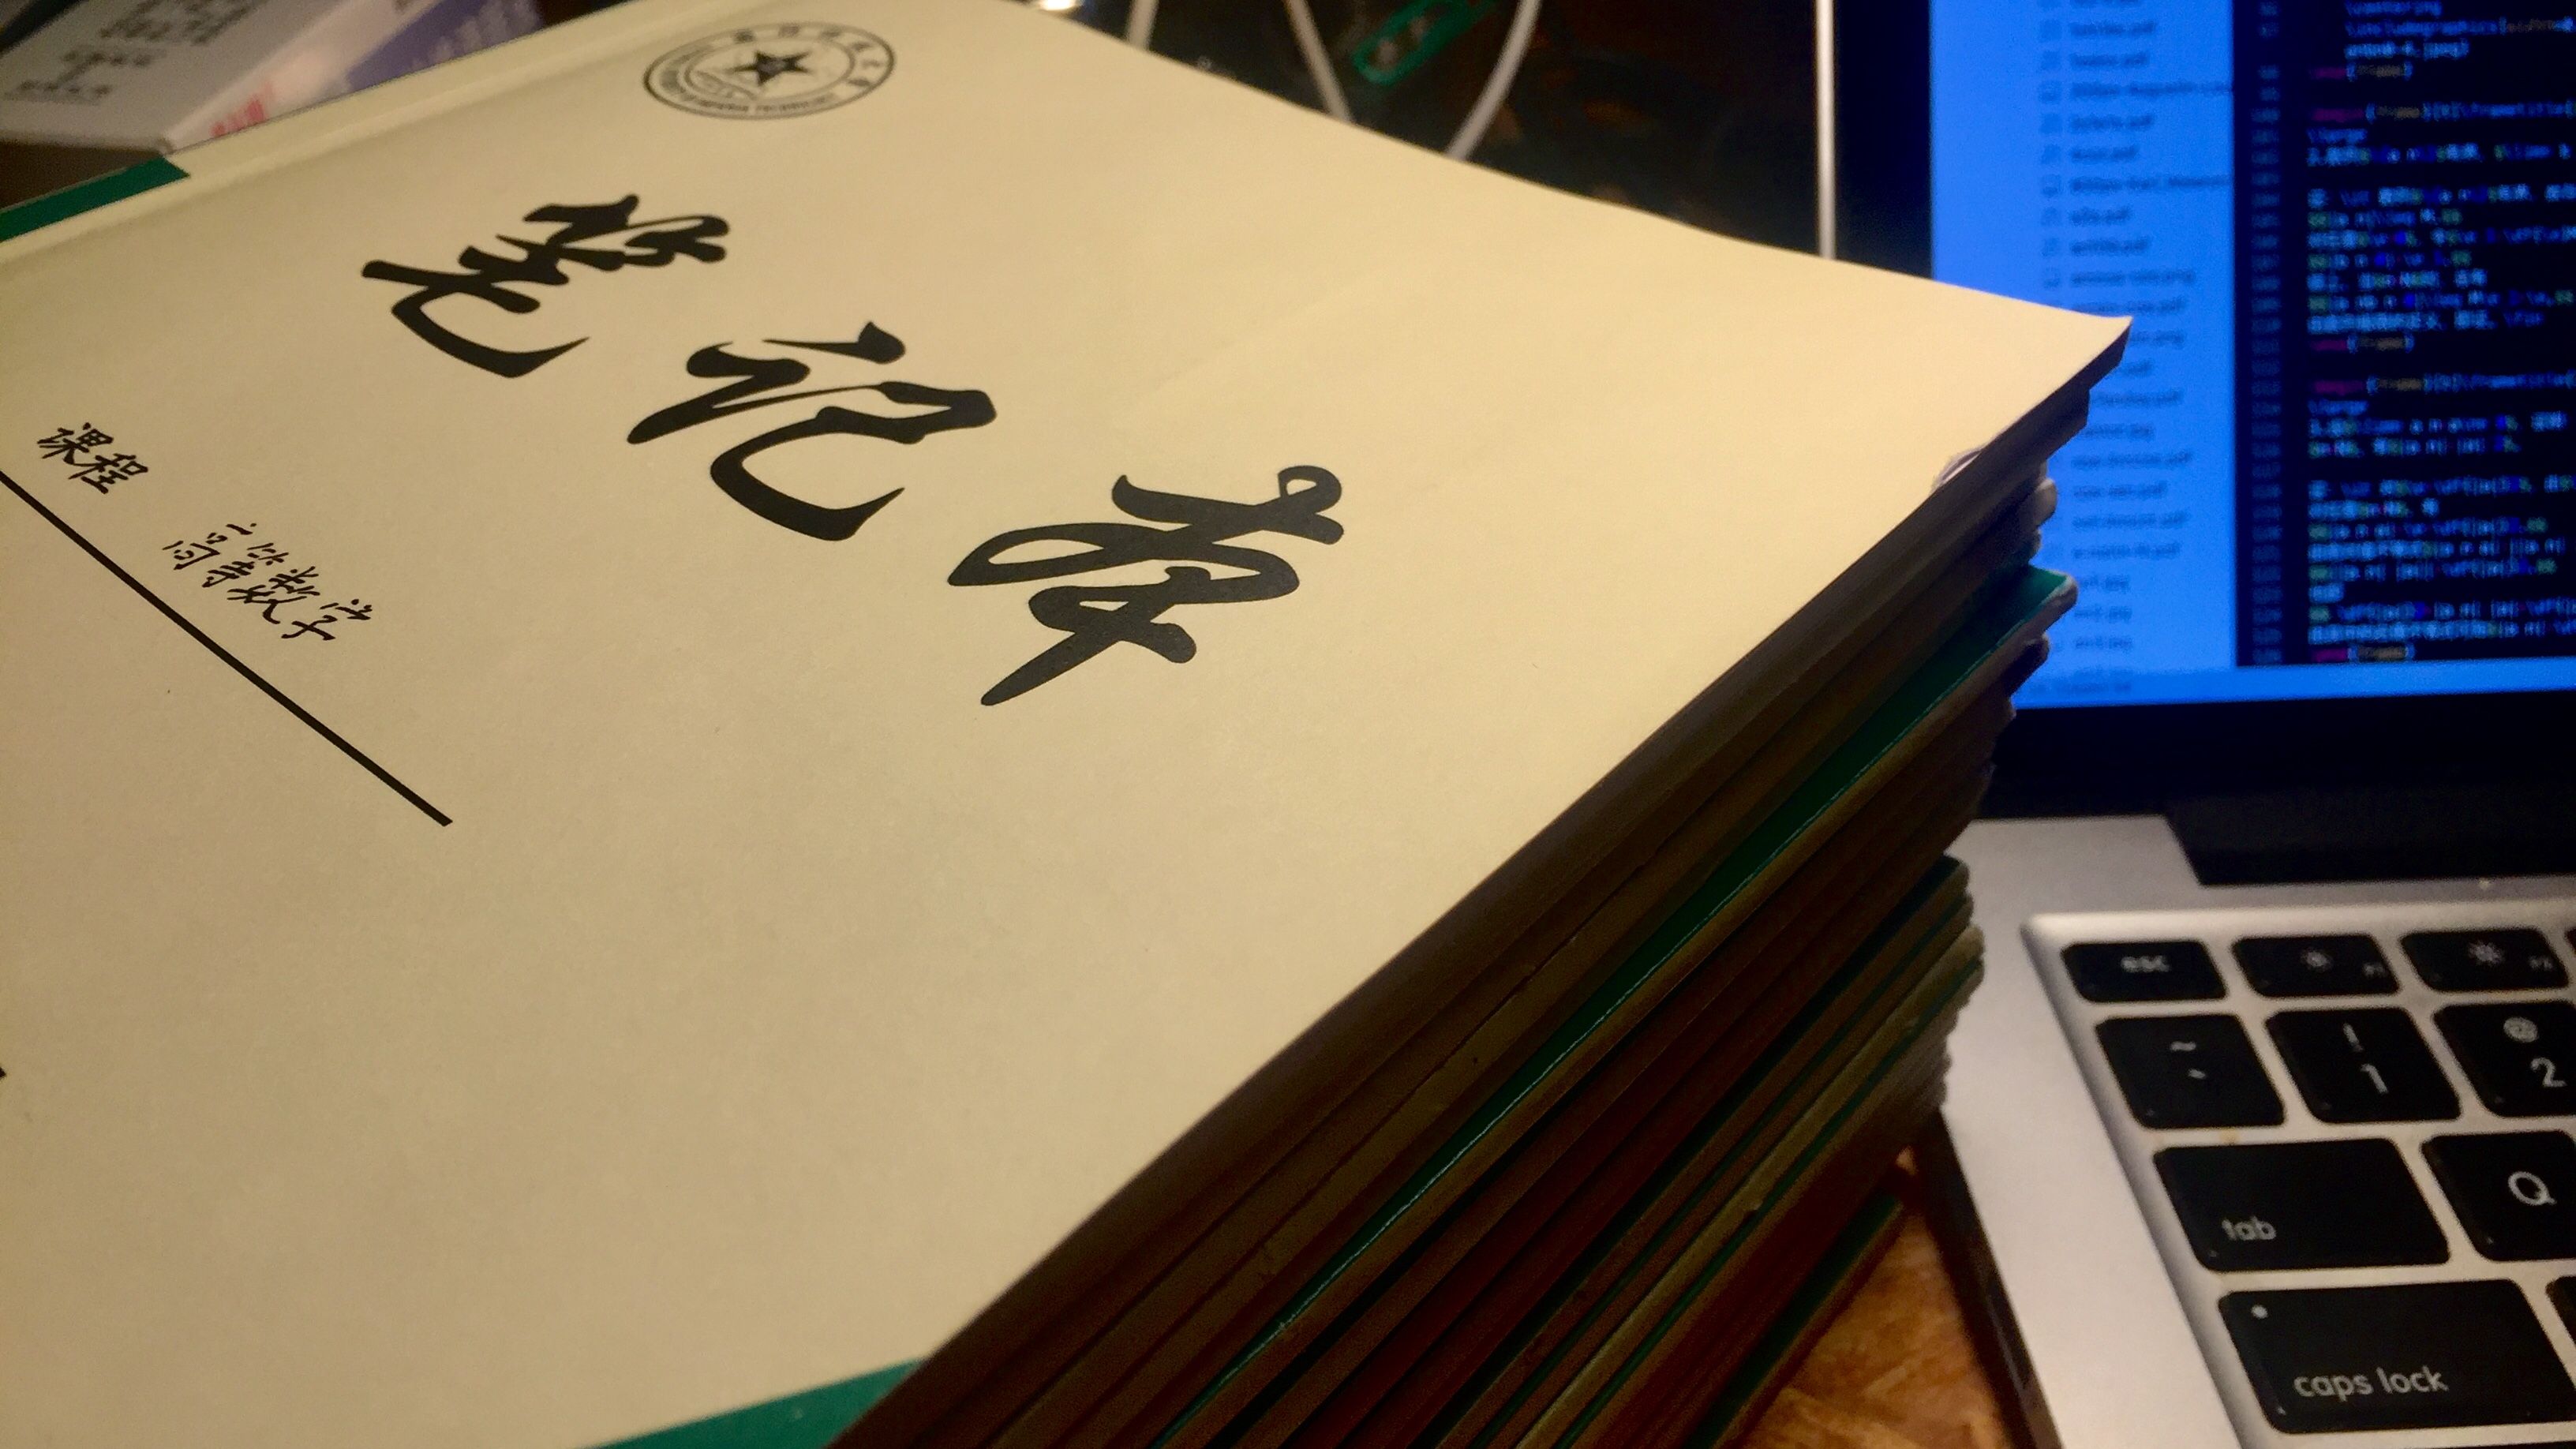
\includegraphics[width=\textwidth]{./images/ch01/HWR/notebook.jpg}

	\begin{flushright}
		\color{white}\vspace*{-2cm}
		\Huge\bf Q \& A
	\end{flushright}
\end{frame}

\end{document}